\documentclass[tikz,border=10pt]{standalone}
\usepackage{tikz}
\usetikzlibrary{angles,quotes,calc, intersections, arrows.meta} % Add this for angle labels

\usetikzlibrary{decorations.markings}
\tikzset{%
  ->-/.style={decoration={markings, mark=at position 0.5 with {\arrow{>}}},
              postaction={decorate}},
  ->>-/.style={decoration={markings, mark=at position 0.5 with {\arrow{>>}}},
               postaction={decorate}},
}
\begin{document}
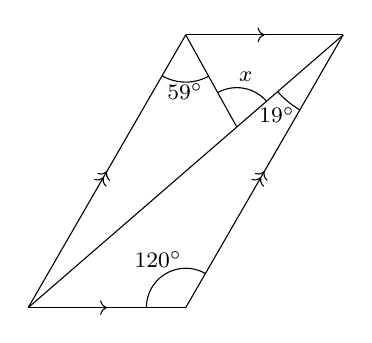
\begin{tikzpicture}[scale = 1]

    % Define the points of the parallelogram
    \coordinate (A) at (0,0);
    \coordinate (B) at (2,0);
    \coordinate (C) at ($(B)+(60:4cm)$); 
    \coordinate (D) at ($(A)+(60:4cm)$); 

    %edges of parallelogram
    \draw[->-] (A) -- (B);
    \draw[->>-] (B) -- (C);
    \draw[->-] (D) -- (C);
    \draw[->>-] (A) -- (D);
    
    %diagonal
    \path[name path=diagonal] (A) -- (C);
    \draw (A) -- (C);

    \path[name path=line1] (D) -- +(-61:4cm);
   
    \draw[name intersections={of=line1 and diagonal,by={Int1}}] (D) -- (Int1);

     % Draw the angle between lines
    \pic [draw, "\footnotesize $120^{\circ}$ ", angle eccentricity=1.4, angle radius=0.5cm] {angle = C--B--A};
    \pic [draw, "\footnotesize $19^{\circ}$", angle eccentricity=1.2, angle radius=1.1cm] {angle = A--C--B};
    \pic [draw, "\footnotesize $59^{\circ}$", angle eccentricity=1.2, angle radius=0.6cm] {angle = A--D--Int1};
    \pic [draw, "\footnotesize $x$", angle eccentricity=1.3, angle radius=0.5cm] {angle = C--Int1--D};

\end{tikzpicture}

\end{document}